\subsection{Làm cho Mạch Có Thể Kiểm Thử (Making Circuits Testable)}
Một mạch được coi là \textit{có thể kiểm thử} nếu các bài kiểm thử có thể được tạo ra cho nó một cách hiệu quả, mạch có thể được kiểm thử với độ phủ lỗi (fault coverage) cao, và thời gian kiểm thử sản phẩm là hợp lý. Tính kiểm thử bao gồm khả năng điều khiển và quan sát. Một mạch sẽ trở nên dễ kiểm thử hơn bằng cách tăng cường hai yếu tố này.

\subsubsection{Sự đánh đổi (Tradeoffs)}
Việc cải thiện khả năng điều khiển và quan sát hầu như luôn đòi hỏi phải chèn thêm phần cứng vào thiết kế. Điều này đồng nghĩa với việc gia tăng số lượng chân cắm (pins), tăng trễ tín hiệu (delays), tăng tiêu thụ năng lượng (power consumption), và tất nhiên là chi phí diện tích phần cứng (hardware overhead). 

Tuy nhiên, bù lại, thiết kế sẽ đạt được độ phủ lỗi tốt hơn và thời gian kiểm thử giảm thiểu. Việc giảm thời gian kiểm thử của một linh kiện sau sản xuất là mục tiêu quan trọng nhất của các kỹ thuật DFT. Nhiệm vụ của kỹ sư thiết kế là phải tối ưu hóa phần cứng được thêm vào sao cho các chi phí đi kèm là thấp nhất.

\subsubsection{Kiểm thử Mạch Tuần tự (Testing Sequential Circuits)}
Một trong những đóng góp quan trọng nhất của DFT là làm cho mạch tuần tự (sequential circuits) có thể kiểm thử được. Việc tạo mẫu kiểm thử hoàn chỉnh cho một mạch tuần tự vô cùng phức tạp và ngay cả khi có, việc áp dụng chúng đòi hỏi quá nhiều chu kỳ xung nhịp để mạch đi vào các trạng thái kích hoạt lỗi.

Kỹ thuật DFT thay đổi cấu trúc của mạch tuần tự sao cho các kỹ thuật kiểm thử mạch tổ hợp có thể được áp dụng lên nó.  

\paragraph{Mô hình Huffman cho Mạch Tuần tự}
Như đã trình bày, mạch tuần tự được mô hình hóa bằng một khối tổ hợp cùng với phản hồi thông qua các phần tử trễ (đối với mạch đồng bộ, đó là các flip-flop có xung nhịp). Đầu vào và đầu ra sơ cấp của mạch chỉ kết nối vào phần tổ hợp. Tín hiệu đồng hồ (clock), set, reset chỉ tác động vào flip-flop phản hồi. Mô hình này tách biệt hoàn toàn các thanh ghi (registers) và phần mạch tổ hợp (buses, khối logic, toán học, ...).

\begin{figure}[H]
    \centering
    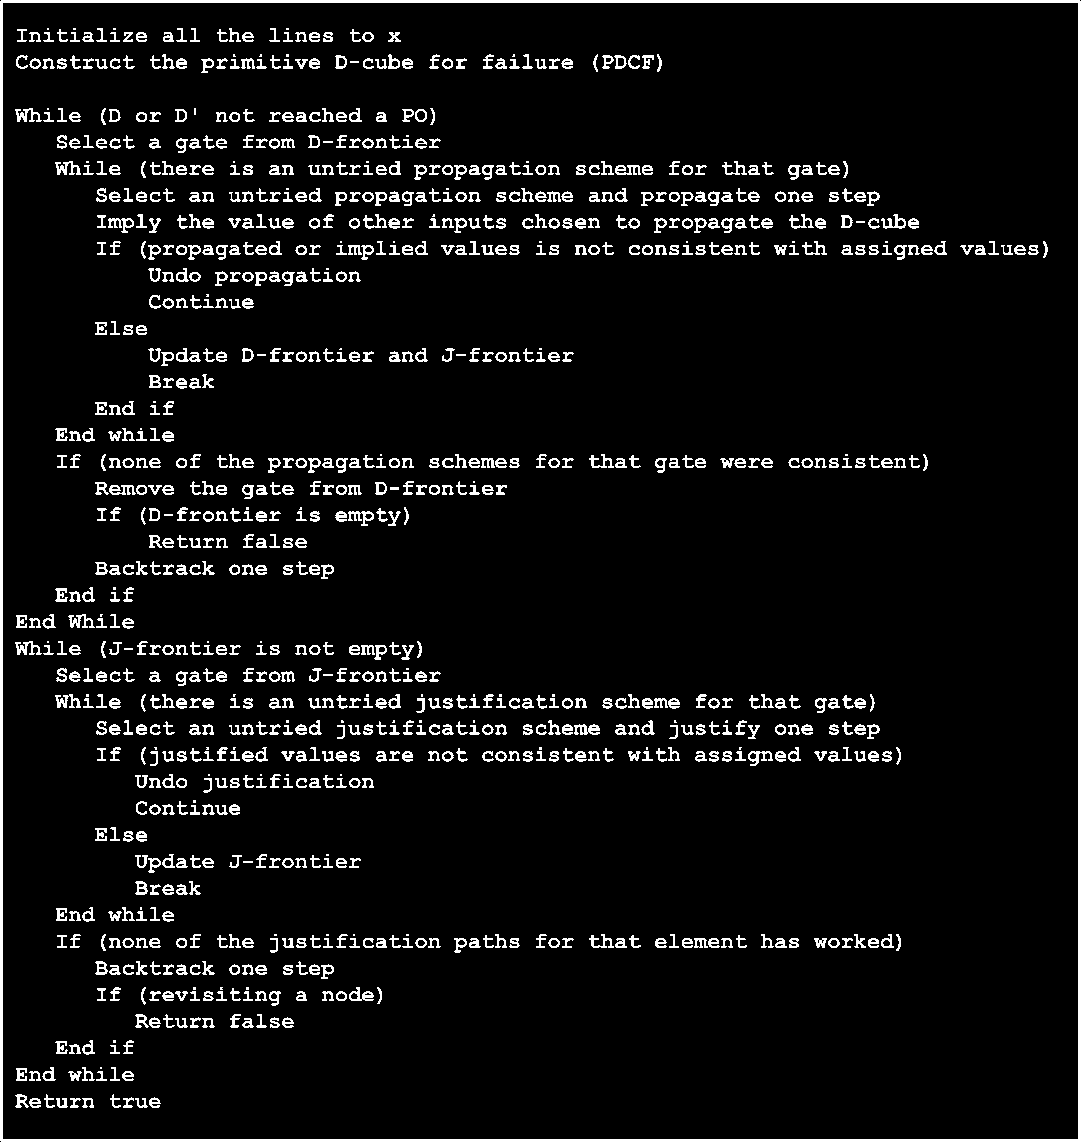
\includegraphics[width=0.7\textwidth]{images/HuffmanCircuitModel.png}
    \caption{\textit{Mô hình Huffman cho kiểm thử (Huffman model for test)}}
\end{figure}

\paragraph{Mô hình Mạch Trải phẳng (Unfolding Sequential Model)}
Mô hình trải phẳng (Unfolded circuit model) phân tách bạch các thanh ghi (phần tuần tự) và phần tổ hợp. Các đầu ra của thanh ghi trở thành "đầu vào giả" (pseudo inputs - PPI) cho mạch tổ hợp, và đầu vào của thanh ghi trở thành "đầu ra giả" (pseudo outputs - PPO). Do đa phần các cổng logic của mạch nằm ở phần tổ hợp, nên việc kiểm thử phần này và tính luôn các cổng vào ra tĩnh của thanh ghi sẽ bao quát được đa số lỗi của thiết kế.

\begin{figure}[H]
    \centering
    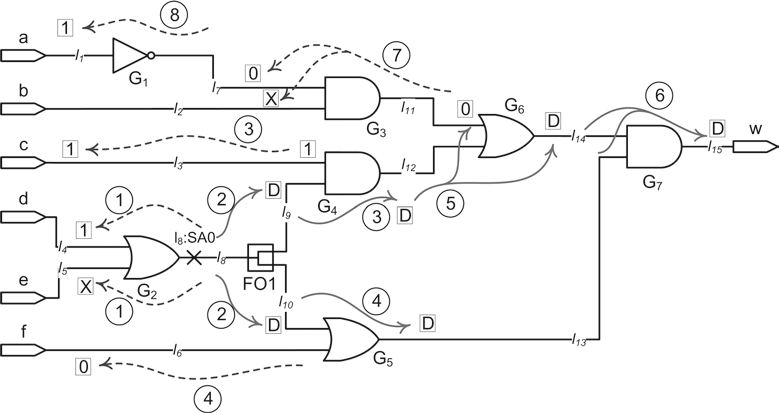
\includegraphics[width=0.7\textwidth]{images/UnfoldedCircuitModel.png}
    \caption{\textit{Mô hình mạch trải phẳng (Unfolded circuit model)}}
\end{figure}

Kết quả kiểm thử trên mô hình trải phẳng sẽ được sử dụng bởi các thiết bị kiểm thử tự động (ATE) để kiểm tra mạch thực tế. Đoạn mã Verilog mô phỏng môi trường kiểm thử này được gọi là một "virtual tester" (thiết bị kiểm thử ảo).

\subsubsection{Tính kiểm thử của Mạch Tổ Hợp (Testability of Combinational Circuits)}
Các mạch tổ hợp cũng hưởng lợi từ DFT. Bằng cách chèn thêm phần cứng, số lượng vector kiểm thử có thể giảm xuống hoặc độ phủ lỗi được tăng lên.

\paragraph{Mô hình lỗi logic (Logic Fault Models)}
Để làm rõ tại sao cần nâng cao tính kiểm thử và áp dụng các kỹ thuật như SCAN (Quét) sau này, ta cần định nghĩa các mô hình lỗi cơ bản có thể xảy ra trong quá trình sản xuất vi mạch:
\begin{itemize}
    \item \textbf{Lỗi kẹt (Stuck-at Faults):} Đây là loại lỗi phổ biến nhất. Một đường tín hiệu/node logic bị "kẹt" cố định ở mức logic 0 (Stuck-at-0) hoặc mức logic 1 (Stuck-at-1), bất kể giá trị kích thích đầu vào thay đổi ra sao.
    \item \textbf{Lỗi trễ (Transition/Delay Faults):} Lỗi không phải về mức logic tĩnh mà là về mặt thời gian. Khối logic chuyển đổi trạng thái quá chậm khi đi từ 0 lên 1 (Slow-to-Rise) hoặc từ 1 xuống 0 (Slow-to-Fall), không đáp ứng được yêu cầu về chu kỳ xung nhịp.
    \item \textbf{Lỗi chập (Bridging Faults):} Xảy ra khi hai hoặc nhiều đường dây tín hiệu vốn độc lập lại vô tình bị ngắn mạch (shorted) với nhau do sai sót trong quá trình gia công vật lý.
\end{itemize}

Trong mạch tuần tự, các trạng thái lưu trữ nội bộ (ẩn trong Flip-flops) khiến việc thiết lập trạng thái và quan sát đầu ra để phát hiện các lỗi trên trở nên vô cùng khó khăn. Đó là lý do căn bản thúc đẩy sự ra đời của kỹ thuật SCAN Design (Thiết kế Quét).
